\subsection{Review}

\subsubsection{Bounds on Intersection Size}

\begin{theorem}[Corr\'adi 1969]
	Let $A_1,\dots,A_n$ be $r$-element sets and $X$ be their union. If $|A_i\cap A_j|\leq k$ for all $i\neq j$, then
	$$|X|\geq\frac{r^2N}{r+(N-1)k}$$
\end{theorem}

\begin{proof}
	Simple counting.
\end{proof}

\begin{theorem}[Erd\"os 1964]
	Let $X$ be a set of $n$ elements $x_1,\dots, x_n$ and let $A_1,\dots, A_n$ be $N$ subsets of $X$ of average size $n/w$. If $N\geq 2kw^k$, then there exist $A_{i_1},\dots,A_{i_k}$ such that
	$$|A_{i_1}\cap\dots\cap A_{i_k}|\geq \frac{n}{2w^k}.$$
\end{theorem}

\begin{proof}
	Simple counting, Jensen's inequality.
\end{proof}

\subsubsection{Graphs with no 4-cycles}

\begin{theorem}[Reiman 1958]
	If $G=(V,E)$ on $n$ vertices has no $4$-cycles, then
	$$|E|\leq \frac{n}{4}(1+\sqrt{4n-3}).$$
\end{theorem}
\begin{proof}
	Uses the `cherry-counting' technique, where the inequality follows from counting the number of `cherries' each vertex can be the midpoint of, and the number of cherries each pair of vertices can form the endpoint of. Both have different bounds.
	
	\begin{figure}[h]
		\centering
		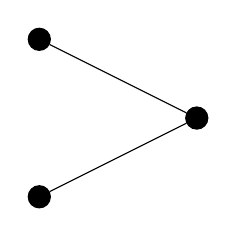
\begin{tikzpicture}
			\node[shape=circle,draw=black,fill=black,inner sep=0pt,minimum size=8pt] (A) at (-1,1) {};
			\node[shape=circle,draw=black,fill=black,inner sep=0pt,minimum size=8pt] (B) at (1,0) {};
			\node[shape=circle,draw=black,fill=black,inner sep=0pt,minimum size=8pt] (C) at (-1,-1) {};
			
			\path [-] (A) edge node[] {} (B);
			\path [-] (C) edge node[] {} (B);

		\end{tikzpicture}
		\caption{A Cherry.}
	\end{figure}
\end{proof}

\subsubsection{Graphs with no induced $4$-cycles}

If you can get $G'$ from $G$ by deleting vertices and ALL edges attached to that vertex from $G$ then $G'$ is an induced subgraph. If you cannot, then $G$ is weakly $G'$-free. We denote $\omega(G)$ to be the number of vertices in the biggest complete subgraph of $G$.

\begin{theorem}
	If an $n$-vertex graph $G=(V,E)$ is weakly $C_4$-free, then 
	$$\omega(G)\geq 0.4\frac{|E|^2}{n^3}.$$
\end{theorem}
\begin{proof}
	Long and complex, look at page 27-29.
\end{proof}

\subsubsection{Zarankiewicz's Problem}

The Zarankiewicz problem asks how many entries an $n\times n$ binary matrix can contain so that it has no $a\times b$ submatrix with all-$1$ entries. This is equivalent to asking the maximum number of edges in a $K_{a-b}$-free bipartite graph.

Let $k_{a,b}(m,n)$ be the number of edges of a maximum $K_{a,b}$-free graph on $m,n$ vertices.

\begin{theorem}[K\H{o}v\'ari, S\'os and Tur\'an]
	For all natural numbers $n\geq a\geq 2$, we have
	$$k_{a,,b}(m,n)\leq (a-1)^{1/b}nm^{1-1/b}+(b-1)m.$$
\end{theorem}

\begin{proof}
	Cherry-counting, except this time you count stars (one vertex in $V_1$ and all other vertices in $V_2$).
\end{proof}

\begin{theorem}[Ossowski 1993]
	Let $G=(V_1,V_2,E)$ be a bipartite graph with no isolated vertices, $|E|<(k+1)^r$ edges and $d(y)\leq r$ for all $y\in V_2$. Then we can delete at most $k$ vertices from $V_1$ so that the resulting graph has no $(r-a+1)\times a$ clique for $a=1,2,\dots,r$.
\end{theorem}




\subsubsection{Omitted Details}

Some filling-in-the-details here, in order to make sure that I'm completely understanding what's happening.

\textbf{Page 29, Prop. 2.8.} The final inequality follows from the averaging principle, but it's not as immediate as meets the eye. We basically use the fact that the elements of $\mathcal{F}$ form a partition of the vertices of $G$, and the fact that every single one of them is a clique. In particular, for any $X,Y\in\mathcal{F}$, the edges from $X$ to $Y$ are not \textit{complete}, and hence $X\cup Y$ is not a clique (also because of the independence of $\alpha$, none of the subsets are cliques either). This means that this is a complete characterization of \textit{all the cliques} in the graph. We then get that the average size of a clique is
$$\frac{1}{|\mathcal{F}|}\sum{X_i\in\mathcal{F}}|X_i| = \frac{n}{|\mathcal{F}|}$$
and it follows from the averaging principle there exists some clique with size greater than or equal to the average clique, and hence
$$\omega(G)\geq\frac{n}{|\mathcal{F}|}.$$

\subsection{Problems}

\paragraph{Question 2.1} Start with the sets $A_i$ and construct new sets $A_{i,j}=A_i\cap A_j$ and $A_i' = A_i\setminus(\cap_{j\neq i} A_j)$. For each $i$, $A_i = A_i'\cup (\cup_{j\neq i} [A_i\cap A_j])$. Then by the union bound we have
$$|A_i|\leq |A_i'|+\sum_{i\neq j}|A_i\cap A_j|$$
and it follows that 
$$\sum_{i=1}^m |A_i| \leq \sum_{i=1}^m |A_i'| + \sum_{i}\sum_{j\neq i}|A_i\cap A_j|$$
Since $|A_i\cap A_j|\leq t$, we have the latter half of the RHS to be $\leq t\binom{m}{2}$. For the former, we notice that $A_i'\cap A_j'=\emptyset$ by definition. Then $\sum_{i=1}^m |A_i'|\leq n$. We have
$$\sum_{i=1}^m |A_i|\leq n + t\binom{m}{2}.$$

\begin{center}
	\line(1,0){70}
\end{center}

\paragraph{Question 2.3} (Did this \textit{without} the hint, very happy.) 

Let $d(x)$ be the degree of $x$ in $\mathcal{F}$. Then $p(x)=d(x)^2 + (m-d(x))^2$. This is because the first condition is satisfied by all $(A,B)$ such that $x$ is in both of them, ie. exactly $d(x)$ of them, while the latter is satisfied by $(A,B)$ such that $x$ is in neither of them. We can expand this to write $p(x) = 2d(x)^2 + m^2 - 2md(x) = m^2 - 2d(x)(m-d(x))$. Now $d(x)(m-d(x))\leq m^2/4$ (which can be easily checked \textbf{--} it reaches its maximum at $d(x)=m/2$) and we have $p(x)\geq m^2-2(m^2/4)=m^2/2$.

\begin{center}
	\line(1,0){70}
\end{center}

\paragraph{Question 2.7} We argue using induction. Suppose that every $(r-1)$-partite $2$-clique free graph contains $\leq 2m^{r-1-1/2^{r-2}}$ edges. The proposition is trivially true for $r=1$.

Consider now an $r$-partite graph with more than $2m^{r-1/2^{r-1}}$ vertices. We can write any $r$-partite graph $G$ as as a subset of the cartesian product $X \times V = V_1\times\dots\times V_{r-1}\times V$. Define the sets $A_v=\{x\in X:(x,v)\in G\}$; we will apply the lemma to them. Clearly the size of $X$ is at most $m^{r-1}$, and so the size of any $A_v$ is at most $m^{r-1}$, and since $v\in V$ we have that the number of such sets is at most $m$. We calculate the average size of the sets as $m^{r-1}/m$, which is $m^{r-2}$. 

Taking $w=\frac{1}{2}m^{1/2^{r-1}}$, we can apply the lemma to find two sets $A_i$ and $A_j$ such that their intersection is of size more than
$$\frac{n}{2w^{2}}=\frac{2m^{r-1}}{m^{1/2^{r-2}}}=2m^{r-1-1/2^{r-2}}.$$
Then $A_i\cap A_j$ must contain a $2$-clique. But this $2$-clique is connected to $i$ and $j$, and hence there is an $m$-partite $2$-clique in this graph.

\begin{center}
	\line(1,0){70}
\end{center}

\paragraph{Question 2.8} This is nearly identical to that of the in-text question of chapter 1, but slightly involved. The double counting trick works.

\begin{center}
	\line(1,0){70}
\end{center}

\paragraph{Question 2.10} Let $A_1,\dots, A_N$ be subsets of some $n$-element set $X$, and suppose that these sets have average size at least $\alpha n$. Show that for every $s\leq (1-\epsilon)\alpha N$ with $0<\epsilon<1$, there are indices $i_1, i_2,\dots, i_s$ such that 
$$|A_{i_1}\cap\dots\cap A_{i_s}|\geq (\epsilon\alpha)^sn.$$

\paragraph{Answer.} (The ideas are correct, but this is unfortunately quite poorly written; I should've been doing this on paper instead of trying to work it out in my head.)

Consider the bipartite graph $(X, V, E)$ where $V = [N]$ and $x\in A_i\iff (x,i)\in E$. Since the size of each $A_i$ is at least $\alpha n$, the number of edges is at least $\alpha nN$. For any family of $s$ sets $\{A_{i_j}\}_{j\in[s]}$, every element in the intersection forms a $(1, s)$-star. By preceding as in the proof of 2.10, we can bound the number of stars as
$$n\binom{|E|/n}{a}\leq \sum_{x\in V}\binom{d(x)}{a}$$
which, setting $a=s\leq (1-\epsilon)\alpha N$ and $|E|=\alpha nN$ gives us
$$n(\alpha N - (1-\epsilon)\alpha N)^s\leq\sum_{x\in V}\binom{d(x)}{s}$$
which gives 
$$n(\epsilon\alpha N)^s\leq \sum_{x\in V}\binom{d(x)}{s}.$$
By expanding the factorial and using $n!/(n-s)!\leq n^s$, we can set
$$n(\epsilon\alpha N)^s\leq \sum_{x\in V} d(x)^s$$
The latter, however, on applying the problem 2.8, gives us
$$n(\epsilon\alpha N)^s\leq\sum_{(i_1,\dots, i_s)}|A_{i_1}\cap\dots\cap A_{i_s}|\leq \binom{N}{s}|A_{i_1}\cap\dots\cap A_{i_s}|$$
where we take the intersection of the largest size to be $(i_1,\dots,i_s)$. We can again use the factorial inequality to get
\begin{align*}
	n(\epsilon\alpha N)^s&\leq N^{s}|A_{i_1}\cap\dots\cap A_{i_s}|\\
	n(\epsilon\alpha)^s&\leq |A_{i_1}\cap\dots\cap A_{i_s}|.
\end{align*}

\begin{center}
	\line(1,0){70}
\end{center}

\paragraph{Question 2.11} This is almost trivial. Consider blocks of size less than $a/b$. Clearly the number of elements in them is at most $ma/b\leq |X|/b$. It immediately follows that blocks of size at most $a/n$ can contain at most $|X|/b$ elements, which means that at least $(1-1/b)|X|$ elements are in blocks of a greater size.

\begin{center}
	\line(1,0){70}
\end{center}

\paragraph{Question 2.12}